\section{Modellalkotás, irodalomkutatás}

Munkámban elsősorban a különböző fűtési típusok közti különbségeket szeretném megvizsgálni. A ház modelljét először adottnak venném, az eltérést pedig a különböző fűtési módok jelentenék.
Azaz megpróbálom felírni a környezet belső hőmérsékletre való ráhatását, eztán pedig modellezem többféle fűtőtest viselkedését.

Ehhez először áttekintettem a hőátadás lehetséges formáit és forrásait. Arra jutottam, hogy ha a levegő hőmérsékletére szabályzok, akkor az abba beleszóló tényezőket veszem sorra:
\begin{itemize}[noitemsep,topsep=0pt,parsep=0pt,partopsep=0pt]
	\item konvektív hőátadás: a felszín közelében felmelegedett levegő áramlani kezd
	\item radiatív hőátadás: sugárzással kibocsátott energia a környezetbe
\end{itemize}

\begin{figure}[h]
	\centering
	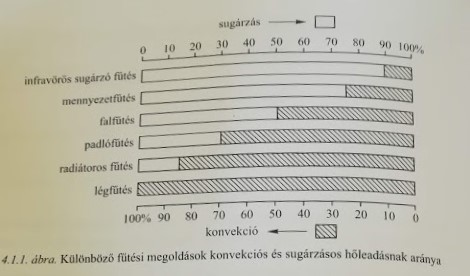
\includegraphics[width=8cm]{figures/konvrad}
	\caption{Alacsony hőmérsékletű fűtés és magas hőmérsékletű hűtés c. könyv ábrája}
		%\footnote{Jan Babiak, rehva Guidebook No.7}
\end{figure}


A levegő hőmérsékletére ezek a következőképp hatnak a leginkább:
\begin{itemize}[noitemsep,topsep=0pt,parsep=0pt,partopsep=0pt]
	\item a fűtőtestek konvektív és radiatív hőátadással is melegítik a környezetet
	\item a radiatív energiát a tárgyak, falak nyelik el, amik ezáltal felmelegszenek (mintegy kapacitásként lesz egy hőtároló tömeg, ami a fűtés kikapcsolásával fenntartja a hőmérsékletet / lassítja a hűlést)
	\item a fűtetlen falfelületek hűtik a szobát (külső hőmérséklet befolyása)
\end{itemize}

Így a kezdeti modellben azzal a feltételezéssel élek, hogy ezen kívül más hatás nem lép fel.

A modellben feltételezem, hogy a fűtőtest felületi hőmérsékletével tudunk beavatkozni. A modellben paraméter a fűtőtestek hőátadási tényezője és felülete. Zavarásként (?) hat a külső hőmérséklet értéke, amit mérni is tudunk. Kimenet a belső hőmérséklet (térben konstansnak véve azt / átlagolva a szoba levegőjére)

A modell felírásához a fűtőtest tulajdonságain kívül szükség van a szobában található levegő mennyiségére is. A zavarás hatását is fel kell írni, azaz hogy egy külső hőmérsékletváltozás hogyan jelenik meg a kimeneten. (Célszerű itt egy átviteli függvényt felírni először, szuperpozíciószerűen. A zavarás viszont nem a modell bemenetén és nem is a kimenetén hat.)

A felírandó átviteli függvények:

\begin{itemize}[noitemsep,topsep=0pt,parsep=0pt,partopsep=0pt]
	\item levegő felmelegedése konstans külső hőmérsékletet feltételezve, fűtőtest egységugrással
	\item levegő felmelegedése fűtés kikapcsolt állapota mellett, környezeti hőmérséklet ugrásával
\end{itemize}

\pagebreak

\subsection{Radiátor modelljének felírása}

Mivel a Matlab szimulációban a legbefúvásos fűtés modelljének teljesítmény kimenete van, fel akartam állítani egy olyan modellt, ami beillesztehető az eredeti légbefúvó rendszer helyére. A ház hőveszteségeit a Matlab számolja\footnote{Pontosításra szorul ez a modell is, mert valószínűleg csak a konvektív hővezetéssel számol (a sugárzásival pedig nem). A légbefúvás a ház levegőjét melegíti. Ám a modellben a ház hőtároló tömege nem jelenik meg, csak egy hőellenállás a veszteségek modellezéséhez.}, ebből pedig adódik a szoba levegőjének hőmérséklete. A rendszer szabályozását így visszavezettem a leadott teljesítmény szabályzására. A levezetett egyenletnek köszönhetően egy teljesítményigényhez meg tudom majd mondani hogy mennyire kell a szabályzószelepeket kinyitni.

%Angol nyelvű szakirodalomból pl. Gouda2000 alapján számolva irreális teljesítményértékeket kaptam (150kW), tovább keresve magyar nyelvű irodalmat is áttekintettem.

Az \textit{Épületgépészet a gyakorlatban}\footnote{Könyvtári könyv, Verlag. 5.11.6, 2. o.} c. könyvben szó esik fűtési rendszerek méretezéséről. Itt adatként szerepel egy épületre a szobák hőigénye\footnote{Pontosan nem tudom még, hogyan definiálják a hőigényt: mekkora kültéri hőmérsékletet vesznek pl. figyelembe, illetve hogy radiátor méretezésénél ezt nyilván felül kell becsülni.} és névleges hőmérséklete. Ehhez választanak megfelelő méretű radiátort, hogy azokban a kiszámolt sebességgel vizet keringetve a hőleadás elég legyen az adott helyiségbe.
{\scriptsize(Ehhez figyelembe kell venni minden radiátorra a keringő víz hőmérsékletét is, különösen ha azok sorba vannak kötve és a hőmérsékletesések is jelentősek.)}
% Adottnak véve az előremenő és visszatérő hőmérsékletet az összes hőigényből számolható a víz kívánt áramlási sebessége. Ezután meghatározzák a radiátorok méretét, hogy azoknak a hőleadása megfeleljen az előírtaknak.

%A fenti példák segítenek a modellalkotásban is, felírható a radiátorok teljesítménye változó vízhőmérséklet és víz tömegáram esetén is. Természetesen a modell egyik bemenete, ez esetben a tömegáram a szabályzott mennyiség. Felteszem, hogy ezt folytonosan tudjuk szabályozni egy szelep segítségével (vagy ha ez nem életszerű, akkor kétállású szeleppel, de nagyobb frekvenciával, mint ahogy egy kazánt tudnánk ki/be kapcsolni).

Hasonlóan méretezési feladatot mutat be a \cite[4.2.7.3]{Herz} is. Ezek alapján vezettem le a leadott hő mennyiségét állandósult állapotra. Természetesen a felmelegedés és lehűlés idejét is figyelembe kell majd venni, de ezzel érthető módon a méretezésnél sem számolnak.%További egyszerűsítésként elhanyagoltam a hőleadási tényező hőmérsékletfüggését is.
%Itt a hőveszteség adott. Esetünkben ezt a házra a Matlab számolja és jól méretezett rendszert tételezünk fel. Csupán azért kell a hőleadást jól felírni, hogy a felfutás, hőkapacitás, stb. során átadott energiát is belekalkuláljuk.

%Persze ilyenkor egyedi esetekből indulok ki, de remélhetőleg ez paraméterezhetően elvezet az általános, többféle házra alkalmazható megoldáshoz.

\subsubsection{Hőleadás}
A fűtőtestek hőleadását befolyásolja a fűtőtestek közepes hőmérsékletkülönbsége (ld. a \ref{termeszeteshk_359}. egyenletet), a felülete és a hőleadási tényezője.
%(A 86. oldalon $\Delta t_k$, a 358.-on $\Delta t_m$ jelöléssel találkozunk. A \cite[359.~o.]{Herz} ismét változik ugyanannak a jelölése. (\ref{termeszeteshk_359}) Ezutóbbi angol jelölés szimpatikusabb.)
%
Ezek közötti kapcsolatot adja az \ref{holeadas}. egyenlet (\cite[358.~o.]{Herz}-ből): 
\begin{equation} \label{holeadas}
\dot Q_{le} = k_e ~ A_e ~ \Delta t_m
\end{equation}
%
%
ahol
\begin{itemize}[itemsep=6pt,topsep=0pt,parsep=0pt,partopsep=0pt]
\item[] $\dot{Q}_{le}$ [\SI{}{\watt}] a leadott hő
\item[] $k_e$ [\si[per-mode = fraction]{\watt\per\meter\squared\per\kelvin}] hőleadási tényező - ezt hőmérsékletfüggetlennek tekintem.
\item[] $A_e$ [\si{\metre\squared}] a radiátor felülete
\item[] $\Delta t_m$ [\SI{}{\kelvin}] a közepes hőmérsékletkülönbség:
\end{itemize}
%
\begin{equation} \label{termeszeteshk_359}
\Delta t_m = \frac{t_s+t_r}{2} -t_{i}
\end{equation}
ahol
%
\begin{itemize}[itemsep=6pt,topsep=0pt,parsep=0pt,partopsep=0pt]
	\item[] $t_s$ a radiátorba befolyó, $t_r$ az onnan kifolyó víz hőmérséklete \si{\degreeCelsius}-ban
	\item[] $t_i$ a szoba hőmérséklete
\end{itemize}
%
A hőátadási tényező is hőmérsékletfüggő, de ezzel egyelőre nem foglalkozom, állandónak tekintem.
%
%\begin{equation} \label{k_e}
%k_e = \frac{\dot{Q}}{A~ \Delta t_m}
%\end{equation}
%
%A hőteljesítmény hőmérsékletfüggő (361.~o.). Az $x^{1.33}$ az egyenletekben $x~ x^{1/3}$, ebből pedig $ x ~ \sqrt[3]{x}$ formában jelenik meg.
%
%
%Nominálisan $\Delta t_m$ = \SI{60}{\celsius}-ra adott érték a közepes hőmérsékletkülönbség függvényében változik:

\subsubsection{Hőfelvétel}
A vízből felvett hő felírható:

\begin{equation} \label{hofelvetel}
\dot Q_{fel} = c ~ \dot{m} ~ \Delta t
\end{equation}

ahol

\begin{itemize}[itemsep=6pt,topsep=0pt,parsep=0pt,partopsep=0pt]
	\item[] $\dot{Q}_{fel}$ [\SI{}{\watt}] a vízből felvett hő, ami annak lehűléséből adódik
	\item[] $c$ [\si[per-mode = fraction]{\joule\per\kg\per\kelvin}] a víz fajhője
	\item[] $\dot{m}$ [\si[per-mode = fraction]{\kg\per\second}] a víz tömegárama
	\item[] $\Delta t = t_s-t_r$ [\SI{}{\kelvin}] a víz lehűlésének mértéke
\end{itemize}

\subsubsection{Energiamérleg állandósult állapotban}
\textbf{Állandósult állapot} esetén a leadott hő egyenlő a felvettel, mivel akkor nem történik hőfelhalmozás, hőtárolás.
Azaz ekkor a radiátor hőkapacitását nem kell figyelembe vennem.

Beírva a (\ref{termeszeteshk_359})-ba (\ref{holeadas})-t:
\begin{equation} \label{holeadas2}
\begin{aligned}
\dot Q_{le} = k_e ~ A_e ~ \left( \frac{t_s+t_r}{2}-t_i\right) = k_e ~ A_e ~ \left( \frac{t_s+(t_s-\Delta t)}{2}-t_i\right)
\end{aligned}
\end{equation}

Ahol felhasználtuk azt is, hogy $t_r = t_s-\Delta t$, majd $\Delta t$ helyére beírhatjuk a (\ref{hofelvetel})  átrendezett alakját:
\begin{equation} \label{hofelvetel2}
~~\Delta t = \frac{\dot Q_{fel}}{c ~ \dot{m}}
\end{equation}

Beírva (\ref{holeadas2})-ba (\ref{hofelvetel2})-t:
\begin{equation} \label{holeadas3}
\begin{aligned}
\dot Q_{le} ~=~ & k_e ~ A_e ~ \left( t_s-t_i-\frac{\dot Q_{fel}}{c ~ \dot{m}}\right)  \\[18pt]
\dot Q_{le} + \frac{k_e ~ A_e ~ \dot Q_{fel}}{2 ~ c ~ \dot{m}} ~ = ~ & k_e ~ A_e ~(t_s-t_i) \\[24pt]
2 ~ c ~ \dot{m} ~ \dot Q_{le} + k_e ~ A_e ~ \dot Q_{fel} ~ = ~ &  k_e ~ A_e ~ 2~ c~ \dot{m} ~(t_s-t_i)
\end{aligned}
\end{equation}

\textbf{Csak abban az esetben, ha} $\dot Q_{le}=\dot Q_{fel}$:




\begin{equation} \label{holeadas4}
\begin{aligned}
~~~~~~\dot Q (2 ~ c ~ \dot{m} + k_e ~ A_e) & ~=~ 2 ~ k_e ~ A_e ~ c~ \dot{m} ~(t_s-t_i) \\[18pt]
~~~~~~\dot Q &~=~ \frac{2~c~\dot{m}~k_e~A_e}{2 ~c ~ \dot{m} + k_e ~ A_e}~(t_s-t_i)
\end{aligned}
\end{equation}

\subsubsection{Modellparaméterek}












\pagebreak